\documentclass[11pt,twoside,titlepage]{article}
\usepackage[english]{babel}
\usepackage{amsmath}
\usepackage{amsfonts}
\usepackage{graphicx}
\usepackage[font=small, format=hang]{caption}
\usepackage{hhline}
\usepackage{lineno}
\usepackage{fancyhdr}
\usepackage{calc}
\usepackage{url}
\usepackage{natbib}
\usepackage{color}
\usepackage{geometry}
\usepackage{epsfig}
\usepackage{endnotes}
\usepackage{upquote}
\usepackage{natbib}
\usepackage{mdwlist}
\usepackage{subcaption}
\usepackage{floatrow}
\renewcommand{\baselinestretch}{1.2}
\usepackage{geometry}
\geometry{ hmargin=2.5cm, vmargin=2.5cm }
\makeatletter
\def\iffloatpage#1#2{\if@fcolmade #1\else #2\fi}
\makeatother

\pagestyle{fancy}
%\fancyhead[LE,RO]{\iffloatpage{\thepage}{\thepage}}
%\fancyhead[RE]{\iffloatpage{}{{\small \textbf{\nouppercase \leftmark}}}}
%\fancyhead[LO]{\iffloatpage{}{\small \rightmark}}
%\renewcommand{\headrulewidth}{\iffloatpage{0pt}{0.4pt}}
\fancyhead[LE,RO]{\small{\textit{Imperial College London\\Biomedical Eng. Dept.}}}
\cfoot{\thepage}

\setlength{\headheight}{13.6pt}
\setlength{\marginparwidth}{0pt}
\setlength{\marginparsep}{0pt}
\setlength{\evensidemargin}{0pt}
\setlength{\oddsidemargin}{0pt}
%\renewcommand{\topmargin}{\iffloatpage{2pt}{22pt}}
%\renewcommand{\textwidth}{\iffloatpage{13cm}{360pt}}
\setlength{\hoffset}{\paperwidth/2-\textwidth/2-1in}


\renewcommand{\baselinestretch}{1.2}
\newcommand{\HRule}{\rule{\linewidth}{0.5mm}}
\def\dotsim{{\buildrel .\over \sim}}
\newcommand{\definition}{
\textbf{\textcolor{red}{Definition:}}
}
\renewcommand{\thefootnote}{\alph{footnote}}
\begin{document}
%\title{Automated Quality Assessment for Magnetic Resonance Images for Further Study in Alzeihmer's Disease Patients}
%\author{Marc Dupuis}
%\date{\today}
%\maketitle
%\begin{titlepage}
%\begin{center}
%
%{\textbf{Marc Dupuis\\}}
%\vspace*{0.2cm}
%\end{center}
%
%\pagenumbering{roman}
%\end{titlepage}
%\thispagestyle{empty}
\pagenumbering{roman}

\setcounter{page}{0}\pagenumbering{arabic}

%%	SMALL INTRODUCTION
\begin{titlepage}
\begin{center}

% Upper part of the page. The '~' is needed because \\
% only works if a paragraph has started.
\vspace*{4cm}
\Large Seed Scientific Candidate Assignment 1\\[0.5cm]

% Title

{ \huge \bfseries U.S.A. Passenger Airline Study}\\[0.4cm]

% Author and supervisor
Marc \textsc{Dupuis}\\
\small marc.f.dupuis@gmail.com\\
\small (980) 319-4717

\vfill

% Bottom of the page
{\large \today}

\end{center}
\end{titlepage}

\section{Project Specifications and Objectives}

The objective of this project is to investigate US passenger airline data using two datasets provided by Seed Scientific and the online Research and Innovative Technology Administration (RITA).

As stated in the prompt, the goal is to: \textit{demonstrate to Seed Scientific my ability to manage a real-world data set, to communicate and contextualize summary statistics, and, most importantly, my creativity and analytical rigor in generating and testing hypotheses.} Furthermore, it is explicitly stated that the assignment is deliberately unspecific and exploratory by nature.

\section{Introductory Note}

Seed Scientific provided two datasets as CSV files which held information on the carrier identification tags and airport locations. In addition to this, I was directed to the RITA website\footnote{http://www.transtats.bts.gov}, which holds data on US airline passenger flights. The available information is extremely diverse and rich and contains data on departure dates, cities and airline as well as delays, cause of delays and cancellations.

The data from the RITA set is remarkably well organized and complete. There is no unexpected missing data and very little modifications had to be done in order to process the data.

\section{Results}

As an occasional passenger, the first questions that came to mind when I was given the data were: what do passenger flight trends look like? And what are the delay/cancellation trends? 

The number of US domestic flights is illustrated in Figure \ref{fig:Number of Flights} for every month from January 2000 to August 2013. Two traits immediately jump out: a significant drop in flights around September 2001 and a sustained but progressive drop beginning in September 2008 (as marked by the red lines). These two dates match the 9/11 terrorist attacks and the US financial market crash of 2008 respectively. The 9/11 attacks caused an $18.18\%$ drop in flights from September to October and did not fully recover until a sudden surge around January 2003.

The blue lines mark other noticeable, yearly trends. There seems to be a surge in flights in summer and a drop around December (Christmas and New Year's eve). These trends were expected and are common knowledge.

\begin{figure}[h!]
        \centering
                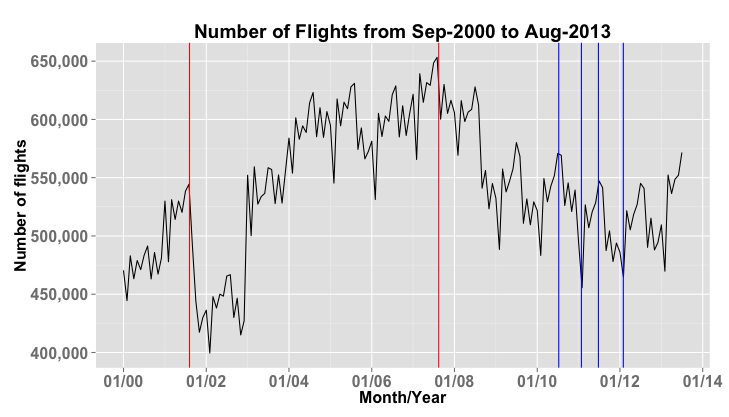
\includegraphics[width=15cm]{Number_of_Flights1.png}
        \caption{Number of US domestic flights from January 2000 to August 2013. The red lines indicate major events (9/11 terrorist attacks and beginning 2008 financial market crash after the subprime mortgage buble) and the blue lines indicate noticeable yearly trends.}\label{fig:Number of Flights}
\end{figure}

Now that we've seen how the number of flights has evolved over the past 13 years, the next question is whether or not delays and cancellations have followed the same trends or if they have been increasing relative to the number of flights (I think we can all agree that it seems like every flight is delayed nowadays.) Fig. \ref{fig:Number of Flights + Delays} is the same as Fig. \ref{fig:Number of Flights} with the delayed and cancelled flights added to the figure. The most remarkable feature of this graph is the ``insignificance'' of the number of cancelled flights relative to the total number of flights, as well as the sudden surge in cancellations around September 2001. Again, this surge marks the time of the 911 attacks. With regards to the delays, these seem to follow the same trends as the total number of flights. Given more time, several more advanced methods would do a better job confirming this, but the correlation between delayed flights and non-delayed flights is approximately $0.68$ versus $0.04$ for cancelled and on-time flights. This shows a rather strong correlation between number of flights and delays and a surprisingly low correlation between cancelled flights and other flights (including delayed flights).

\begin{figure}[h!]
        \centering
                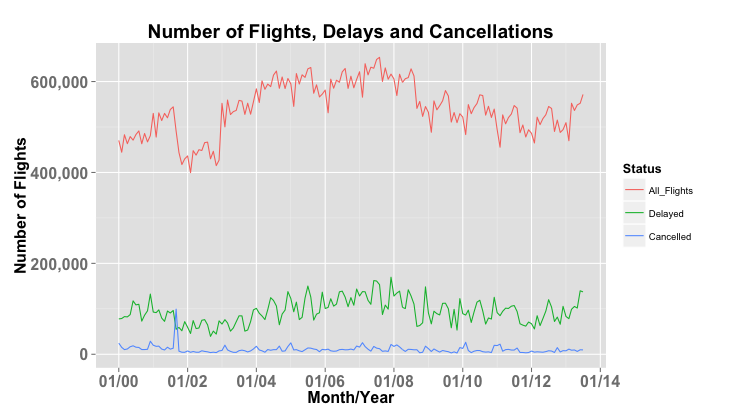
\includegraphics[width=16cm]{Number_of_Flights2.png}
        \caption{Example of Ixico image processing flowchart.}\label{fig:Number of Flights + Delays}
\end{figure}

Following the observations marked by the blue lines in Fig. \ref{fig:Number of Flights}, it would be interesting to look at the number of flights and delays by month (Fig. \ref{fig:Flights by Month}) The bar graph seems to support the idea of an increase of flights in the summer and a drop at the end of each year. However, the delays by month would be better expressed as a percentage of total flights. This is done in Fig. \ref{fig:Flights by Month Percentage}. This bar graph seems to suggest that delays are rather steady with a slight increase around the summer period and Christmas holidays (again, common knowledge).


\begin{figure}[h!]
        \centering
                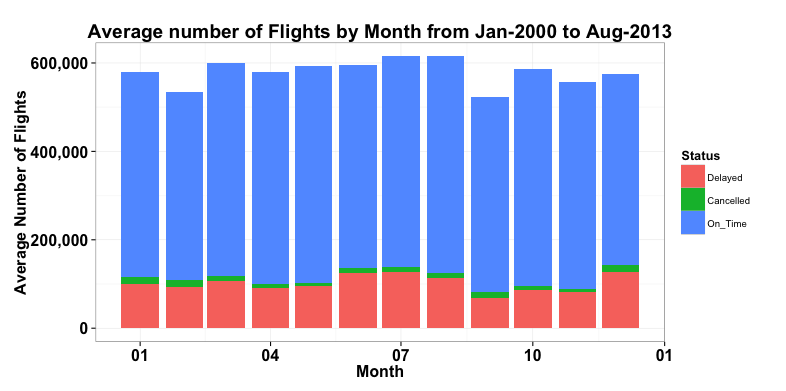
\includegraphics[width=16cm]{Bar1.png}
        \caption{Example of Ixico image processing flowchart.}\label{fig:Flights by Month}
\end{figure}

\begin{figure}[h!]
        \centering
                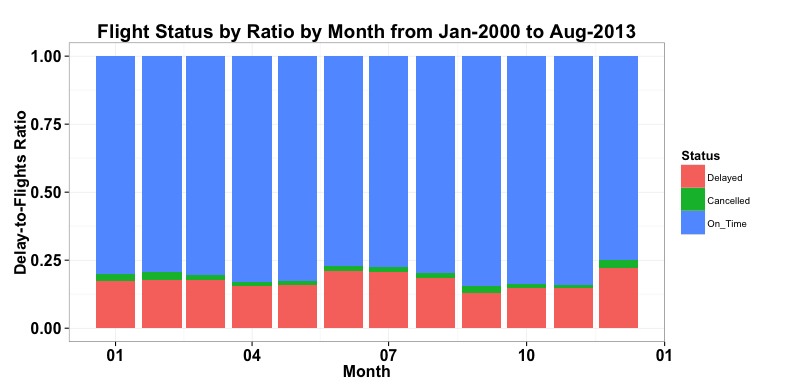
\includegraphics[width=16cm]{Bar2.png}
        \caption{Example of Ixico image processing flowchart.}\label{fig:Flights by Month Percentage}
\end{figure}

\break

Now that we understand more about flight trends and delays/cancellations, it would be interesting to see what the major causes of delays are. Is there one airline that performs better than another? Is it better to depart from a state known for good weather? Fig. \ref{fig:Pie} breaks up the causes of delays into five categories:

\begin{enumerate}\itemsep1pt \parskip0pt \parsep0pt
  \item Late aircraft
  \item National Airspace System (NAS) delay
  \item Carrier delay
  \item Weather
  \item Security
\end{enumerate}

With this figure however, it seems as if weather is not a frequent cause for delay, even though we would intuitively think that it is one of the main causes. This is because the NAS only categorizes delays as due to weather if the weather is severe\footnote{http://www.rita.dot.gov/bts/help/aviation/html/understanding.html}. Minor weather delays fall under NAS orders and thus contribute to the NAS section of the pie chart.

\begin{figure}[h!]
        \centering
                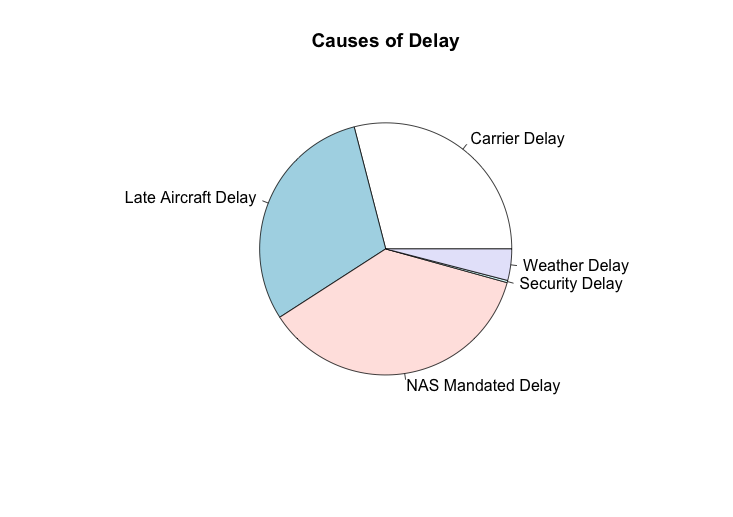
\includegraphics[width=16cm]{Pie.png}
        \caption{Example of Ixico image processing flowchart.}\label{fig:Pie}
\end{figure}



\begin{figure}[h!]
        \centering
                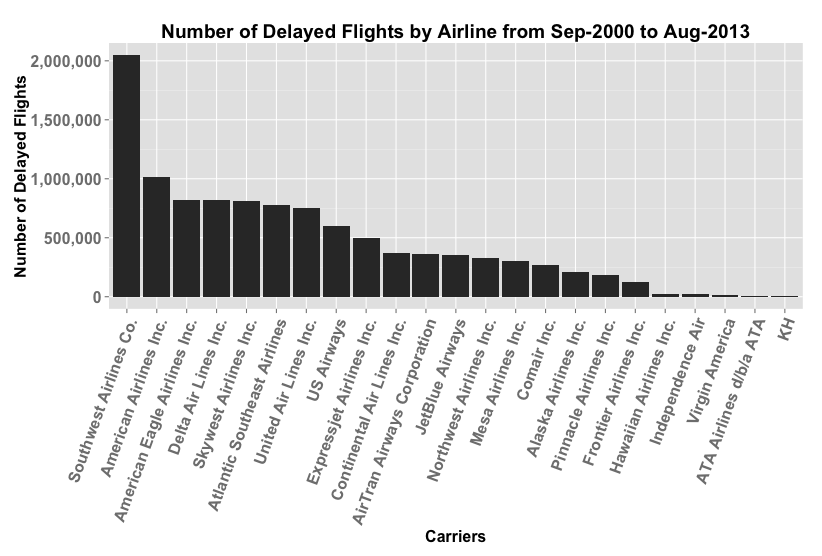
\includegraphics[width=16cm]{Delayed_by_Airline1.png}
        \caption{Example of Ixico image processing flowchart.}\label{fig:flowchart}
\end{figure}

\begin{figure}[h!]
        \centering
                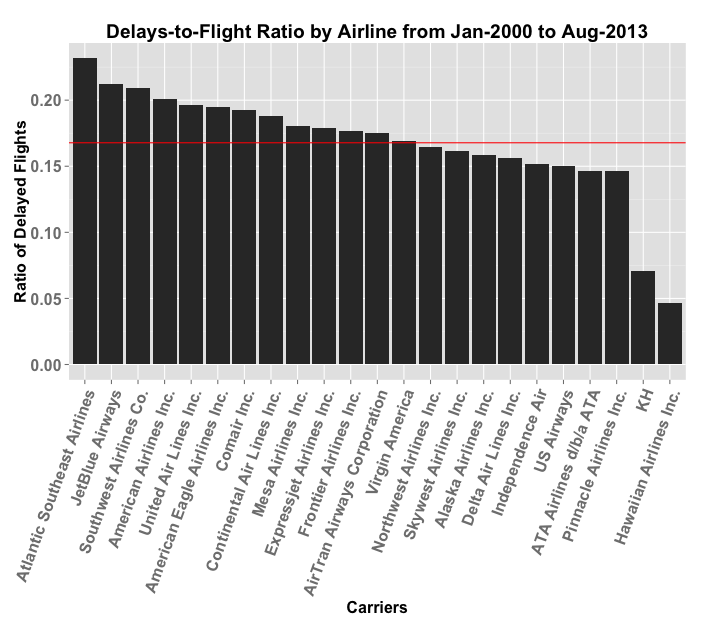
\includegraphics[width=16cm]{Delayed_by_Airline2.png}
        \caption{Example of Ixico image processing flowchart.}\label{fig:flowchart}
\end{figure}

\begin{figure}[h!]
        \centering
                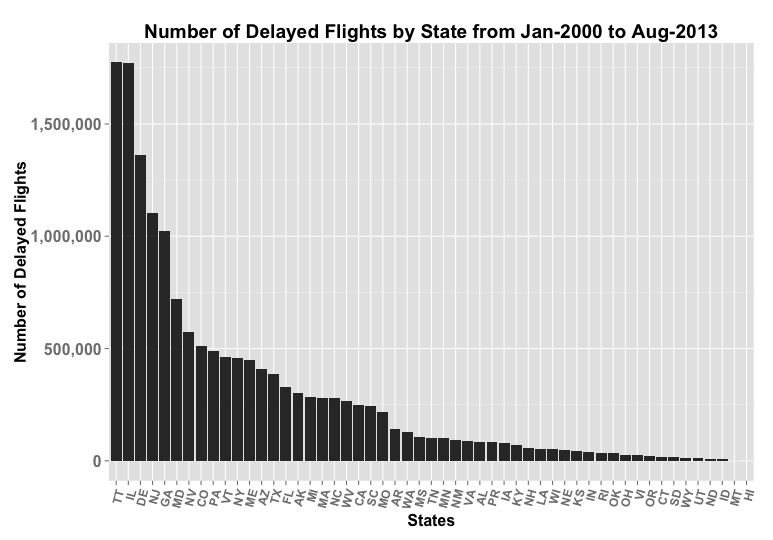
\includegraphics[width=16cm]{Delays_by_State1.png}
        \caption{Example of Ixico image processing flowchart.}\label{fig:flowchart}
\end{figure}

\begin{figure}[h!]
        \centering
                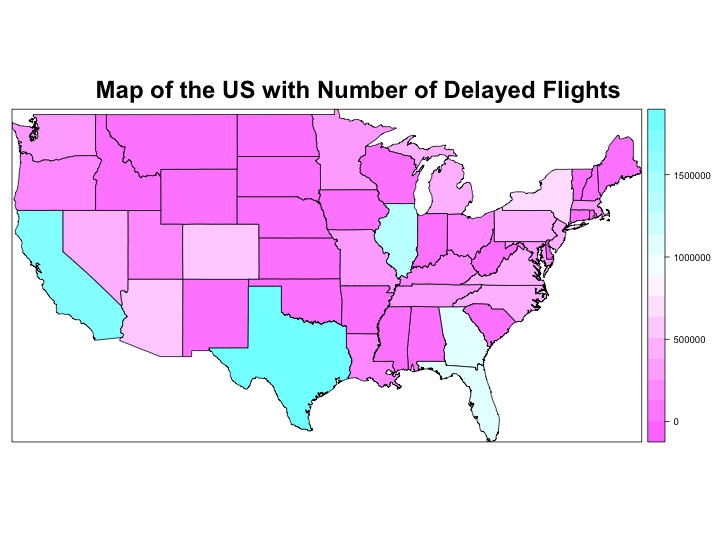
\includegraphics[width=16cm]{USMap1.png}
        \caption{Example of Ixico image processing flowchart.}\label{fig:flowchart}
\end{figure}

\begin{figure}[h!]
        \centering
                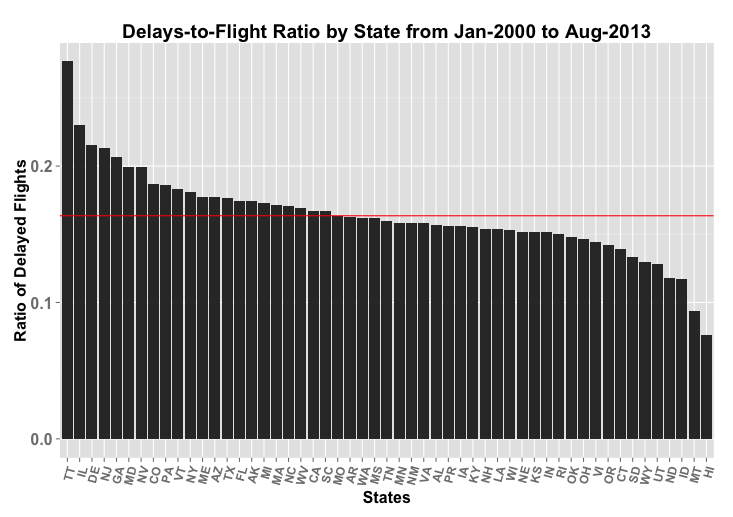
\includegraphics[width=16cm]{Delays_by_State2.png}
        \caption{Example of Ixico image processing flowchart.}\label{fig:flowchart}
\end{figure}

\begin{figure}[h!]
        \centering
                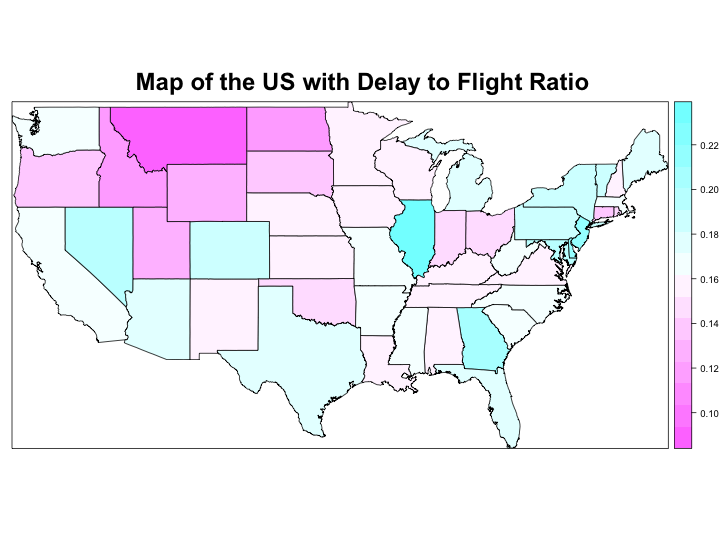
\includegraphics[width=16cm]{USMap2.png}
        \caption{Example of Ixico image processing flowchart.}\label{fig:flowchart}
\end{figure}

\end{document}
